% \iffalse
\let\negmedspace\undefined
\let\negthickspace\undefined
\documentclass[beamer]{IEEEtran}
\usepackage{cite}
\usepackage{amsmath,amssymb,amsfonts,amsthm}
\usepackage{algorithmic}
\usepackage{graphicx}
\usepackage{textcomp}
\usepackage{xcolor}
\usepackage{txfonts}
\usepackage{listings}
\usepackage{enumitem}
\usepackage{mathtools}
\usepackage{gensymb}
\usepackage{comment}
\usepackage[breaklinks=true]{hyperref}
\usepackage{tkz-euclide} 
\usepackage{listings}
\usepackage{gvv}                                        
\def\inputGnumericTable{}                                 
\usepackage[latin1]{inputenc}                                
\usepackage{color}                                            
\usepackage{array}                                            
\usepackage{longtable}                                       
\usepackage{calc}                                             
\usepackage{multirow}                                         
\usepackage{hhline}                                           
\usepackage{ifthen}                                           
\usepackage{lscape}
\usepackage[export]{adjustbox}

\newtheorem{theorem}{Theorem}[section]
\newtheorem{problem}{Problem}
\newtheorem{proposition}{Proposition}[section]
\newtheorem{lemma}{Lemma}[section]
\newtheorem{corollary}[theorem]{Corollary}
\newtheorem{example}{Example}[section]
\newtheorem{definition}[problem]{Definition}
\newcommand{\BEQA}{\begin{eqnarray}}
\newcommand{\EEQA}{\end{eqnarray}}
\newcommand{\define}{\stackrel{\triangle}{=}}
\theoremstyle{remark}
\newtheorem{rem}{Remark}
\begin{document}
\parindent 0px
\bibliographystyle{IEEEtran}

\title{Assignment\\[1ex]10.5.4-2}
\author{ee23btech11215 - Penmetsa Srikar Varma$^{}$% <-this % stops a space
}
\maketitle
\newpage
\bigskip

\renewcommand{\thefigure}{\theenumi}
\renewcommand{\thetable}{\theenumi}
\section*{Question:}
Q10) The sum of three numbers in G.P. is 56. If we subtract 1, 7, 21 from these numbers in that order, we obtain an arithmetic progression. Find the numbers.
\section*{Solution:}
{\centering
Table of Parameters\\
}
\begin{table}[h]
    \centering
    \begin{tabular}{|c|c|}
        \hline
         Input Variable & Condition\\
        \hline
         $x\brak{0}$ & first term of AP\\
         \hline
         $r$ & common ratio of GP\\
         \hline
         $x\brak{0},x\brak{1},x\brak{2}$ & three terms in GP \\
         \hline
         $x\brak{0},x\brak{1},x\brak{2}$ & $x\brak{0}+x\brak{1}+x\brak{2}=56$ \\
         \hline
          $x\brak{0}-1,x\brak{1}-7,x\brak{2}-21$ & form an AP \\
         \hline
          $x\brak{n}$ & $\brak{n+1}^{th}$ term of GP \\
         \hline
         $x\brak{n}\system{Z}X\brak{z}$ & $X\brak{z}=x\brak{0}\sum_{k=0}^{k=\infty}\brak{\frac{z}{r}}^{-k}$\\
         \hline
    \end{tabular}
     \label{tab:t1}
\end{table}
We know that, if three numbers p,q and r are in arithmetic progression then,
\begin{equation}
\label{q1}
2q = p + r
\end{equation}
Then $\brak{n+1}^{th}$ term of GP x\brak{n} is given by:\\

\begin{align}
\label{e1}
x\brak{n}=x\brak{0}.r^{n}
\end{align}

Then from given,
\begin{align}
x\brak{0}+x\brak{1}+x\brak{2}=56
\end{align}

\begin{align}
x\brak{0}.\left(1+r+r^2\right)=56
\end{align}

\begin{equation}
\label{q2}
x\brak{0}\implies\frac{56}{\left(1+r+r^2\right)}
\end{equation}

and from given another case following are in AP,
$$
x\brak{0}-1,x\brak{1}-7,x\brak{2}-21
$$

Then from (\ref{q1}),
\begin{align}2(x\brak{1}-7)=x\brak{0}-1+x\brak{2}-21\end{align}
\begin{align}x\brak{0}\left(r^2-2r+1\right)=8\end{align}
and from (\ref{q2})
\begin{align}\frac{56.\left(r^2-2r+1\right)}{\left(1+r+r^2\right)}=8\end{align}
\begin{align}7\left(r^2-2r+1\right)=\left(1+r+r^2\right)\end{align}
\begin{align}6r^2-15r+6=0\end{align}
\begin{align}2r^2-5r+2=0\end{align}
\begin{align}(2r-1)\ (r-2)=0\end{align}
\begin{equation}
\label{q3}
r=2,\frac{1}{2}
\end{equation}
so from (\ref{q2}),
\begin{align}x\brak{0}=8,32\end{align}
Then from (\ref{e1})
\begin{align}
    \label{a11}
    x_{1}\brak{n}=8.2^{n}=2^{n+3}
\end{align}
\begin{align}
    \label{a12}
    x_{2}\brak{n}=32.\left(\frac{1}{2}\right)^{n}=2^{5-n}
\end{align}\\\\
$x\brak{0}$,$x\brak{1}$ and $x\brak{2}$ are 8,16 and 32 $\brak{or}$ 32,16 and 8 respectively
\begin{figure}[h]
    \centering
    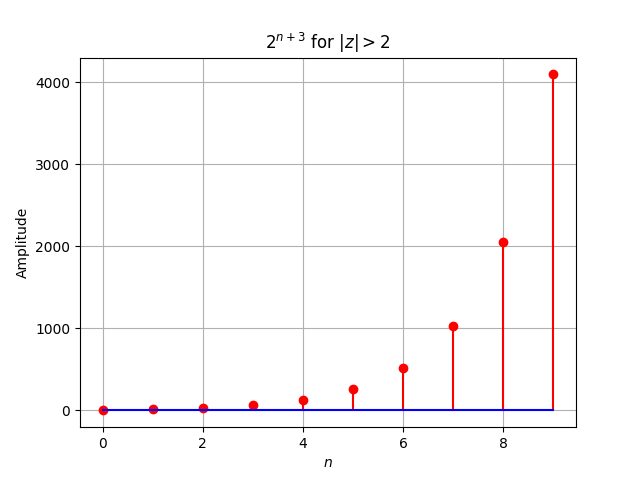
\includegraphics[width=0.5\textwidth]{py_1.png}
    \label{fig:enter-label}
    \caption*{Graph of $2^{n+3}$ }\\
\end{figure}
\begin{figure}[h]
    \centering
    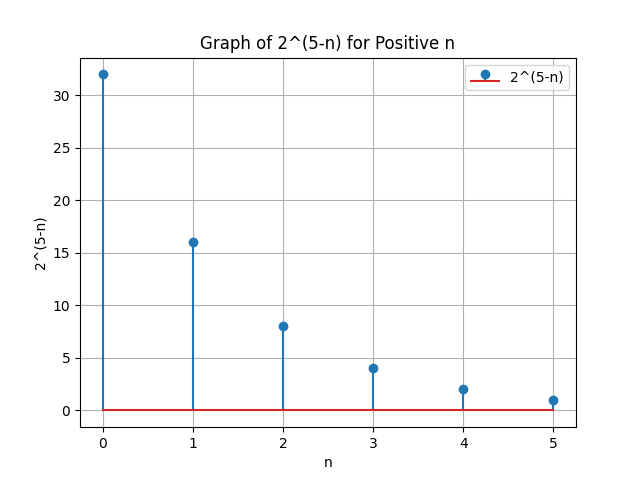
\includegraphics[scale=0.558]{py_2.png}
    \caption*{Graph of $2^{5-n}$}\\
    \label{fig:enter-label}
\end{figure}
We know that Z-Transform of x\brak{n} is given by:
\begin{align}
\label{a13}
    X\brak{z}=\sum_{k=-\infty}^{\infty} x\brak{k}.z^{-k}
\end{align}
where, we assume that x\brak{k}=0   for \brak{k<0}\\
\brak{\ref{a13}} Then, modify as follows:
\begin{align}
\label{a14}
    X_1\brak{z}=\sum_{k=0}^{\infty} x_1\brak{k}.z^{-k}
\end{align}
from \brak{\ref{a11}},
\begin{align}X_1\brak{z}=\sum_{k=0}^{\infty} 8.2^k.z^{-k}\end{align}

\begin{align}X_1\brak{z}=8.\sum_{k=0}^{\infty} \brak{\frac{2}{z}}^k\end{align}

\begin{align}X_1\brak{z}=8.\lim_{n\to\infty} \left(\frac{1-\brak{2.z^{-1}}^{n+1}}{1-2.z^{-1}}\right)\end{align}
Hence,
\begin{align}
X_1\brak{z}=\frac{8}{1-2z^{-1}}\quad if\ \brak{|2z^{-1}|<1}
\end{align}
or,
$$X_1\brak{z}\ is\ undefined\quad if\ \brak{|2z^{-1}|>1}$$
and also from \brak{\ref{a12}},\\
\begin{align}
    X_2\brak{z}=\sum_{k=0}^{\infty} x_2\brak{k}.z^{-k}
\end{align}
\begin{align}X_2\brak{z}=\sum_{k=0}^{\infty} 32.\brak{\frac{1}{2}}^k.z^{-k}\end{align}
\begin{align}X_2\brak{z}=32.\sum_{k=0}^{\infty} \brak{\frac{1}{2z}}^k\end{align}
or,
\begin{align}X_2\brak{z}=32.\lim_{n\to\infty} \left(\frac{1-\brak{\brak{2z}^{-1}}^{n+1}}{1-{\brak{2z}^{-1}}}\right)\end{align}
Hence,
\begin{align}X_2\brak{z}=\frac{32}{1-{\brak{2z}^{-1}}}\quad if\ \brak{|{\brak{2z}^{-1}}|<1}\end{align}
or,
$$X_2\brak{z}\ is\ undefined\quad if\ \brak{|{\brak{2z}^{-1}}|>1}$$
\begin{figure}[h]
    \centering
    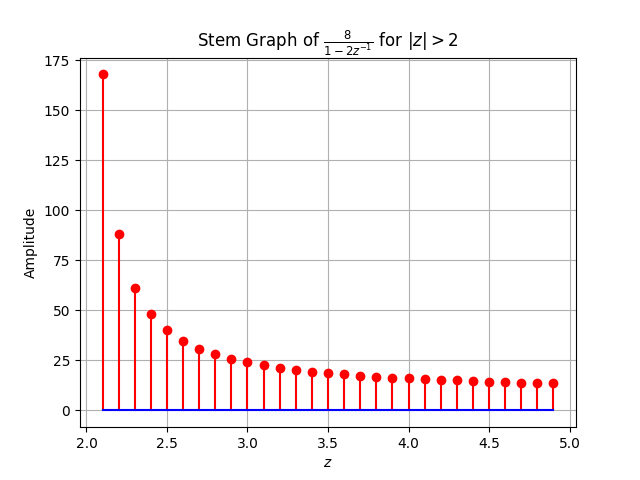
\includegraphics[scale=0.6]{py_11.png}
    \label{fig:enter-label}
    \caption*{Graph of $\frac{8}{1-2Z^{-1}}$}
\end{figure}
\begin{figure}[h]
    \centering
    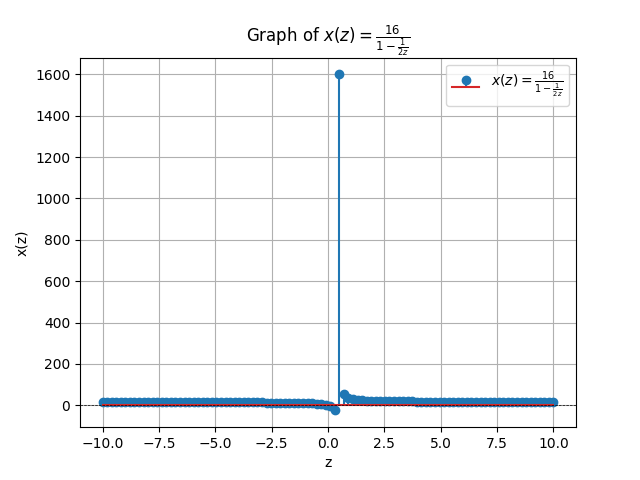
\includegraphics[scale=0.6]{py_12.png}
    \label{fig:enter-label}
    \caption*{Graph of $\frac{32}{1-\left(2Z\right)^{-1}}$}
\end{figure}
\end{document}
